% bei Standalone in documentclass noch:
% \RequirePackage{luatex85}

\documentclass[captions=tableheading, titlepage= firstiscover, parskip = half , bibliography=totoc]{scrartcl}
%paper = a5 für andere optinen
% titlepage= firstiscover
% bibliography=totoc für bibdateien
% parskip=half  Veränderung um Absätze zu verbessern

\usepackage{scrhack} % nach \documentclass
\usepackage[aux]{rerunfilecheck}
\usepackage{polyglossia}
\usepackage[style=numeric, backend=biber]{biblatex} % mit [style = alphabetic oder numeric] nach polyglossia
\addbibresource{lit.bib}
\setmainlanguage{german}

\usepackage[autostyle]{csquotes}
\usepackage{amsmath} % unverzichtbare Mathe-Befehle
\usepackage{amssymb} % viele Mathe-Symbole
\usepackage{mathtools} % Erweiterungen für amsmath
\usepackage{fontspec} % nach amssymb
% muss ins document: \usefonttheme{professionalfonts} % für Beamer Präsentationen
\usepackage{longtable}

\usepackage[
math-style=ISO,    % \
bold-style=ISO,    % |
sans-style=italic, % | ISO-Standard folgen
nabla=upright,     % |
partial=upright,   % /
]{unicode-math} % "Does exactly what it says on the tin."
\setmathfont{Latin Modern Math}
% \setmathfont{Tex Gyre Pagella Math} % alternativ

\usepackage[
% die folgenden 3 nur einschalten bei documenten
locale=DE,
separate-uncertainty=true, % Immer Fehler mit ±
per-mode=symbol-or-fraction, % m/s im Text, sonst \frac
]{siunitx}

% alternativ:
% per-mode=reciprocal, % m s^{-1}
% output-decimal-marker=., % . statt , für Dezimalzahlen

\usepackage[
version=4,
math-greek=default,
text-greek=default,
]{mhchem}

\usepackage[section, below]{placeins}
\usepackage{caption} % Captions schöner machen
\usepackage{graphicx}
\usepackage{grffile}
\usepackage{subcaption}

% \usepackage{showframe} Wenn man die Ramen sehen will

\usepackage{float}
\floatplacement{figure}{htbp}
\floatplacement{table}{htbp}

\usepackage{mhchem} %chemische Symbole Beispiel: \ce{^{227}_{90}Th+}


\usepackage{booktabs}

 \usepackage{microtype}
 \usepackage{xfrac}

 \usepackage{expl3}
 \usepackage{xparse}

 % \ExplSyntaxOn
 % \NewDocumentComman \I {}  %Befehl\I definieren, keine Argumente
 % {
 %    \symup{i}              %Ergebnis von \I
 % }
 % \ExplSyntaxOff

 \usepackage{pdflscape}
 \usepackage{mleftright}

 % Mit dem mathtools-Befehl \DeclarePairedDelimiter können Befehle erzeugen werden,
 % die Symbole um Ausdrücke setzen.
 % \DeclarePairedDelimiter{\abs}{\lvert}{\rvert}
 % \DeclarePairedDelimiter{\norm}{\lVert}{\rVert}
 % in Mathe:
 %\abs{x} \abs*{\frac{1}{x}}
 %\norm{\symbf{y}}

 % Für Physik IV und Quantenmechanik
 \DeclarePairedDelimiter{\bra}{\langle}{\rvert}
 \DeclarePairedDelimiter{\ket}{\lvert}{\rangle}
 % <name> <#arguments> <left> <right> <body>
 \DeclarePairedDelimiterX{\braket}[2]{\langle}{\rangle}{
 #1 \delimsize| #2
 }

\setlength{\delimitershortfall}{-1sp}

 \usepackage{tikz}
 \usepackage{tikz-feynman}

 \usepackage{csvsimple}
 % Tabellen mit \csvautobooktabular{"file"}
 % muss in table umgebung gesetzt werden


% \multicolumn{#Spalten}{Ausrichtung}{Inhalt}

\usepackage{hyperref}
\usepackage{bookmark}
\usepackage[shortcuts]{extdash} %nach hyperref, bookmark

\newcommand{\ua}[1]{_\symup{#1}}
\newcommand{\su}[1]{\symup{#1}}


\title{Versuch 354}
\subtitle{Gedämpfte und erzwungene Schwingungen}
\author{Sebastian Pape\\
        sepa@gmx.de \and
        Jonah Nitschke\\
        lejonah@web.de}
\date{Durchführung: 01.02.2017\\
      Abgabe: 08.02.2017}

\begin{document}

\maketitle
\newpage

\section{Theorie}

In dem folgenden Versuch wird ein elektronischer Kreis, im Kern bestehend aus einem
Widerstand, einer Spule und einem Kondensator betrachtet. Mit Hilfe dieser Schaltung kann eine
gedämpfte Schwingung betrachtet werden, sowie durch Anschluss eines Generators
eine erzwungene Schwingung. Im Laufe des Versuches sollen der Dämpfungswiderstand,
die Frequenzabhängigkeit der Kondensatorspannung sowie die Phase zwischen
Erreger- und Kondensatorspannung betrachtet werden.

\subsection{Der gedämpfte Schwingkreis}

Der in diesem Experiment betrachtete gedämpfte Schwingkreis ist im Grunde nur
eine Erweiterung des RC-Kreise mit einer Spule. Somit kommen in der Schaltung
zwei Energiespeicher vor, zwischen denen die Energie hin und her schwingt. Durch
den eingebauten Widerstand geht bei der Schwingung Energie in Form von Wärme verloren
und somit wird das ganze System gedämpft. Betrachtet man solch eine Schaltung, kann
mithilfe der Kirchhoffschen Gesetze eine Differentialgleichung für den Strom I
mithilfe des Widerstandes R, der Spule L und dem Kondensator C aufgestellt werden:

\begin{equation}
  \frac{\su{d}^2I}{\su{d}t^2} + \frac{R}{L}\frac{\su{d}I}{\su{d}t} + \frac{1}{LC} I = 0 .
\end{equation}

Durch Lösen der Differentialgleichung ergibt sich mit einem geeigneten Ansatz für
die Frequenz ein Term, der von der Stärke der Dämpfung abhängig ist:

\begin{equation}
  \label{eqn:omega1,2}
  \tilde{\omega}_{1,2} = j \frac{R}{2L} \pm \sqrt{ \frac{1}{LC} - \frac{R^2}{4L^2}} .
\end{equation}

Je nachdem wie sich der unter der Wurzel stehende Term verhält, können für die
gedämpfte Schwingung verschiedene Fälle betrachtet werden, von denen zwei im Folgendem
erläutert werden.

\textbf{1.Fall :} $\frac{1}{LC} > \frac{R^2}{4L^2}$

In diesem Fall ist der Term mit der Wurzel rein reel und  es entsteht eine
harmonische Schwingung, deren Amplitude mit zunehmender
Zeit gegen Null geht. Die Einhüllende wird dabei durch eine Exponentialfunktion
beschrieben, wie auch in Abbildung \ref{fig:Schwingfall} anhand der rot gestrichelten
Linie zu sehen ist.
Mithilfe der Schwingungsdauer lässt sich dann errechnen, nach welcher
Zeit die Amplitude auf den $e$-ten Teil ihrer Ursprungsamplitude abgesenkt ist:

\begin{equation}
  \label{eqn:T_ex}
  T\ua{ex} := \frac{2L}{R} \su{s} .
\end{equation}

\begin{figure}
  \centering
  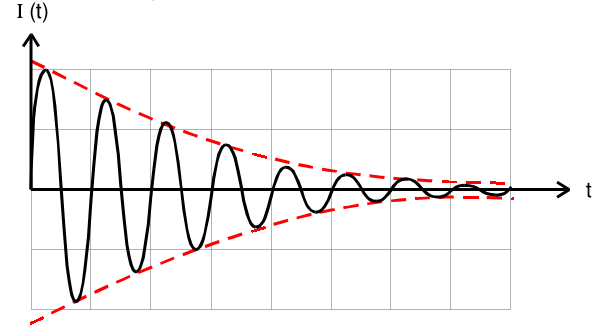
\includegraphics{Schwingfall.png}
  \caption{Zeitlicher Verlauf einer gedämpften Schwingung \cite{anleitung01}.}
  \label{fig:Schwingfall}
\end{figure}

\textbf{2.Fall :} $\frac{1}{LC} < \frac{R^2}{4L^2}$

Bei diesem Fall handelt es sich um eine aperiodische Dämpfung, bei der die Lösung
keinen oszillatorischen Teil besitzt. In diesem Versuch wird dabei nur der als
aperiodischer Grenzfall bezeichneter Spezialfall betrachtet, bei dem
$\frac{1}{LC} = \frac{R^2}{4L^2}$ gilt und der Strom ohne Überschwinger am schnellsten
gegen Null geht (siehe schwarz gestrichelte Linie Abbildung \ref{fig:Kriechfall}).

\begin{figure}
  \centering
  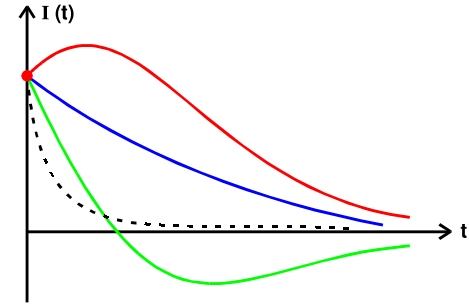
\includegraphics{Kriechfall.png}
  \caption{Möglicher Zeitverlauf des Stromes in einem Schwingkreis mit aperiodischer Dämpfung \cite{anleitung01}.}
  \label{fig:Kriechfall}
\end{figure}

\newpage

\subsection{Die erzwungene Schwingung}

Wird bei dem vorher betrachteten Schaltkreis noch ein Generator kontinuierliche
Spannungsquelle eingebaut,
handelt es sich um eine erzwungene Schwingung. Mithilfe der
Kirchhoffschen Gesetze ergibt sich für die Kondensatorspannung $U\ua{C}$
folgende Differentialgleichung:

\begin{equation}
  LC\frac{\su{d}^2U\ua{C}}{\su{d}t^2} + RC\frac{\su{d}U\ua{C}}{\su{d}t} + U\ua{C} = U\ua{0} \exp^{j\omega t} .
\end{equation}

Aus dieser Differentialgleichung können nun mit einem geeigneten Ansatz eine Funktion
für die Kondensatorspannung $U\ua{c}$ sowie eine Gleichung für die Phasenverschiebung
$\varphi$ zwischen Erreger- und Kondensatorspannung bestimmt werden:

\begin{align}
  \varphi(\omega) &= \arctan \left( \frac{-\omega RC}{1 - LC\omega^2} \right) \\
  U\ua{C}(\omega) &= \frac{U\ua{0}}{ \sqrt{ \left(1 - LC\omega^2 \right)^2 + \omega^2R^2C^2}} .
\end{align}

Die Kondensatorspannung kann bei der sogenannten Resonanzfrequenz $\omega\ua{res}$
auch einen Wert größer als $U\ua{0}$ annehmen:

\begin{equation}
  \label{eqn:omega_res}
  \omega\ua{res} = \sqrt{\frac{1}{LC} - \frac{R^2}{2L^2}} .
\end{equation}

Wird bei der Schaltung eine schwache Dämpfung betrachtet, für die
$\frac{R^2}{2L^2} \, << \, \frac{1}{LC}$ gilt, nähert sich $\omega\ua{res}$
der Kreisfrequenz $\omega\ua{0}$ der ungedämpften Schwingung an. In diesem
Fall übertrifft $U\ua{C}$ die Erregerspannung $U\ua{0}$ um den Faktor
$\frac{1}{\omega\ua{0}RC}$, welcher auch als Güte $q$ des Schwingkreises bezeichnet wird.

Ein weiterer Faktor für die Güte eines Schwingkreises ist die Breite der Resonanzkurve,
welche durch die beiden Frequenzen $\omega\ua{+}$ und $\omega\ua{-}$ charakterisiert
wird. Bei den beiden Frequenzen handelt es sich um die Werte, bei denen die
Kondensatorspannung auf den Bruchteil $\frac{1}{\sqrt{2}}$ ihres Maximalwertes
absinkt. Für Güte und Breite folgt dabei folgende Beziehung:

\begin{equation}
  q = \frac{\omega\ua{0}}{\omega\ua{+} - \omega\ua{-}} .
\end{equation}

\newpage

\section{Durchführung}

Im ersten Teil des Experimentes wird die Zeitabhängigkeit der Amplitude untersucht,
um daraus den effektiven Dämpfungswiderstand zu bestimmen. Dafür wird die Schaltung
aus Abbildung \ref{fig:MessungA} verwendet. Die verwendete Schaltung besteht aus
einem Stromkreis, in dem der Nadelimpulsgenerator, der Widerstand $R\ua{2}$, eine
Spule und ein Kondensator in Reihe geschaltet sind. Unter Verwendung eines Tastkopfes wird die an
dem Kondensator abfallende Spannung auf ein Oszillographen gegeben, auf dem dann
die abklingende Schwingung beobachtet wird.

Mithilfe des Reglers wird die Zeitachseneinstellung so angepasst, bis
auf dem Bildschirm ein Intervall zu sehen ist, auf dem die Amplitude etwa um
den Faktor 3 bis 8 abgenommen hat. Anschließend werden mit der Cursor sowohl
Amplituden der Maxima sowie auch der zeitliche Abstand gemessen und ein Thermodruck
angefertigt.

\FloatBarrier
\begin{figure}
  \centering
  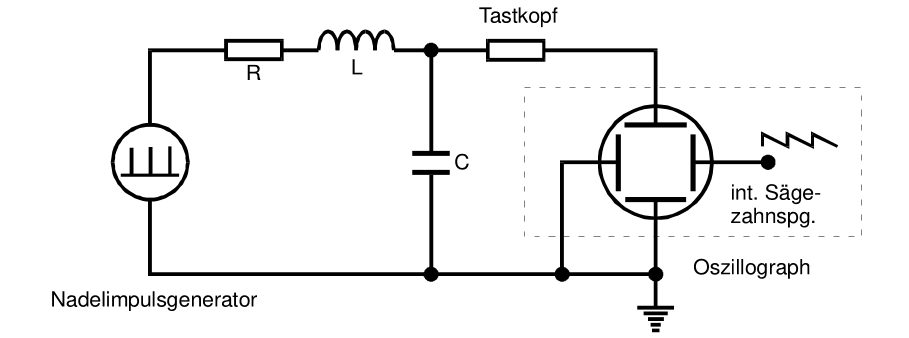
\includegraphics{MessungA.png}
  \caption{Schaltung zur Messung der Zeitabhängigkeit der Kondensatorspannungsamplitude \cite{anleitung01}.}
  \label{fig:MessungA}
\end{figure}
\FloatBarrier


Im zweiten Fall wird die Schaltung aus Abbildung \ref{fig:MessungA} ebenfalls
verwendet, jedoch wird nun anstatt des vorherigen Widerstandes ein variabler
Widerstand mit einem maximalen Wert von 5 $\su{\Omega}$ eingebaut. Der Widerstand wird
zuerst auf seinen maximalen Wert eingestellt, sodass auf dem Bildschirm eine
kritische Dämpfung beobachtbar ist. Dann wird der Widerstand so lange runter geregelt, bis
auf dem Oszilloskop ein Überschwinger zu sehen ist. Der Dämpfungswiderstand ist
dabei genau in dem Moment eingestell, wo gerade noch kein Überschwinger zu erkennen
ist.

\newpage
%\FloatBarrier
%\begin{figure}
%  \centering
%  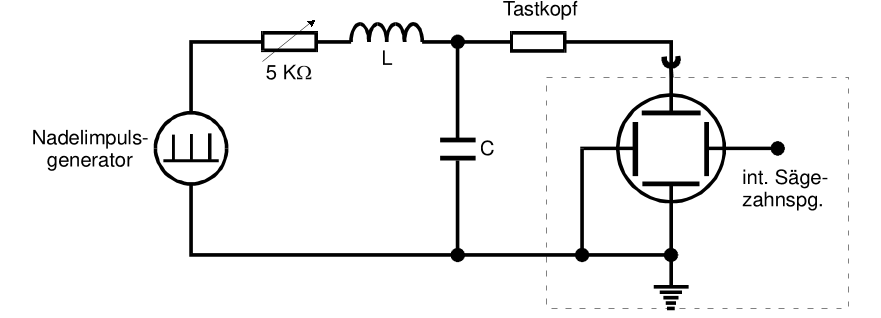
\includegraphics{MessungB.png}
%  \caption{Schaltung zur Bestimmung des Dämpfungswiderstandes bei dem aperiodischen Grenzfall \cite{anleitung01}.}
%  \label{fig:MessungB}
%\end{figure}
%\FloatBarrier

Für die letzten beiden Teile der Messung wird wieder der Schaltplan aus Abbildung
\ref{fig:MessungA} verwendet. Dabei wird der variable Widerstand wieder entfernt
und ein fester Widerstand $R\ua{2}$ in die Schaltung eingebaut. Über den Generator
wird nun eine Sinusspannung in den Stromkreis eingegeben, wobei die Eingangsspannung
nun ebenfalls auf den zweiten Eingang des Oszillographen gegeben wird.
Somit werden auf dem Oszilloskop sowohl die Erreger- als auch die Kondensatorspannung
sichtbar gemacht. Zuerst werden bei jeder Frequenzveränderung die Amplituden beider
Spannungen notiert, wobei die jeweilig eingestellte Frequenz direkt am Generator
abgelesen wird. Dann werden mithilfe des Cursors der zeitliche Abstand der beiden
Nulldurchgänge beider Spannungsverläufe sowie die Wellenlänge der Kondensatorspannung
gemessen, um daraus hinterher die Phasenverschiebung zu berechnen.

%\FloatBarrier
%\begin{figure}
%  \centering
%  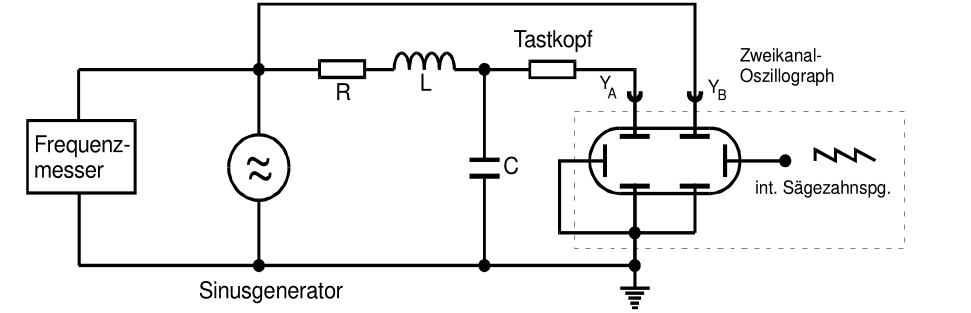
\includegraphics{MessungC.png}
%  \caption{Schaltung zur Messung der Frequenzabhängigkeit sowie der Phasenverschiebung \cite{anleitung01}.}
%  \label{fig:MessungC}
%\end{figure}
%\FloatBarrier

\newpage

\section{Auswertung}

Die verwendeten Zylinder wurden mithilfe einer Schieblehre vermessen und
hatten die folgenden Längen. Dabei werden die Werte als fehlerfrei angenommen.

\begin{description}
  \item[Zylinder 1] \SI{40,35}{\milli\meter}
  \item[Zylinder 2] \SI{80,55}{\milli\meter}
  \item[Zylinder 3] \SI{80,45}{\milli\meter}
  \item[Zylinder 4] \SI{102,1}{\milli\meter}
  \item[Zylinder 5] \SI{31,1}{\milli\meter}
  \item[Zylinder 6] \SI{39,7}{\milli\meter}
  \item[Zylinder 7] \SI{61,5}{\milli\meter}
\end{description}

\subsection{Bestimmung der Dämpfungskonstante und der Schallgeschwindigkeit mit dem Impuls--Echo--Verfahren}

Die Dämpfungskonstante $\alpha$ aus \eqref{eqn:Intensität}
lässt sich aus den genommenen Daten berechnen. Dafür werden die Messdaten
in die Formel \eqref{eqn:Intensität} eingesetzt und wie folgt nach $\alpha$ aufgelöst.

\begin{equation}
  \label{eqn:dämpfung}
  \alpha = - \frac{1}{x_1} \ln{\left(\frac{I_0^\text{'}}{I_0}\right)}
\end{equation}

Dabei ist $I_0^\text{'}$ die Amplitude an der Stelle $x_1 > 0$ und $I_0$
die Amplitude an der Stelle $x  = 0$.

Die Messdaten sind in Tabelle \ref{tab:Messdaten} dargestellt.
Die Werte für Zylinder 4 und den zusammengesetzten Zylinder mit dem
achten Messwert wurden für die Berechnung der Dämpfungskonstante nicht
verwendet, weil die Peaks nur bei Verstärkug ausgemessen werden konnten.
Auf das Herausrechnen des Verstärkungsfaktors wurde der Einfachheit halber verzichtet.
Im Mittel ergibt sich die Dämpfungskontante zu:

\begin{equation}
  \alpha = \SI{21.257(301)}{\per\meter}.
\end{equation}

Der Fehler ist die Standardabweichung des Mittelwertes.
Eine Darstellung der Dämpfung in Acryl ist in dem Diagramm \ref{fig:Dämpfung}
einzusehen. Dabei sind die Messdaten der Anfangs- und Endamplituden
ebenfalls eingetragen.


\begin{figure}
  \centering
  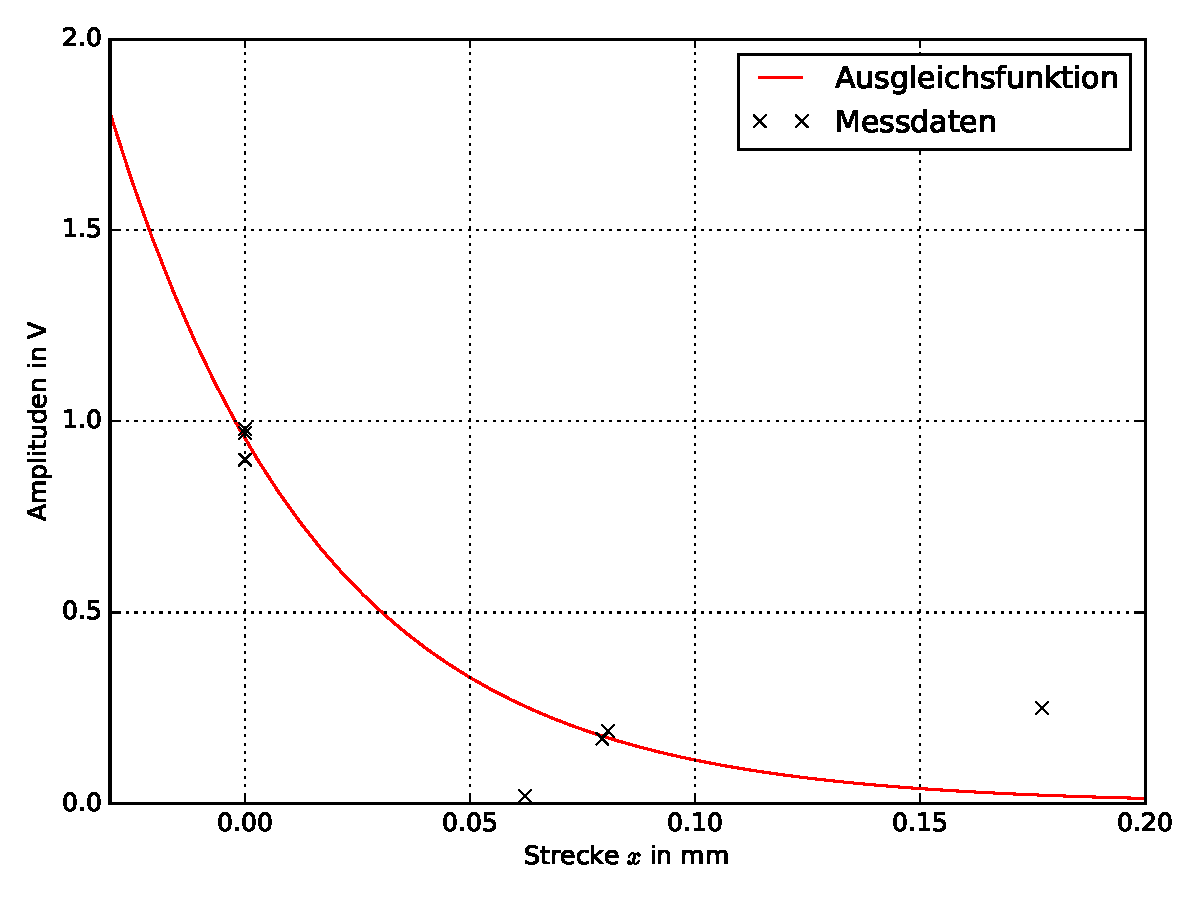
\includegraphics[width=\textwidth]{Pics/Daempfung.pdf}
  \caption{Darstellung der Dämpfung der Amplitude mit Zunahme der Strecke.}
  \label{fig:Dämpfung}
\end{figure}

Die Schallgeschwindigkeit ist aus den Laufzeiten zwischen den
gemessenen Peaks und den vermessenen Zylinderlängen mithilfe von
\eqref{eqn:Fehlstelle} zu berechnen. Dafür wurde mit dem
\emph{Python}-Packet \emph{curve\_fit} eine lineare Ausgleichsrechnung
durchgeführt. Der systematische Fehler der Sonde ist der Ordinaten-Abschnitt
der Ausgleichgeraden und die Schallgeschwindigkeit ist in der Steigung
wiederzufinden.

Die Werte ergeben sich zu:

\begin{align}
  \label{eqn:schallgesch_echo}
  c\ua{Acryl, echo} &= \SI{2880.943}{\meter\per\second} \\
  \Delta\ua{Sonde,echo} &= \SI{-3.862}{\meter\per\second}.
\end{align}

Das zugehörige Diagramm der Messung ist im Folgenden dargestellt.

\begin{figure}
  \centering
  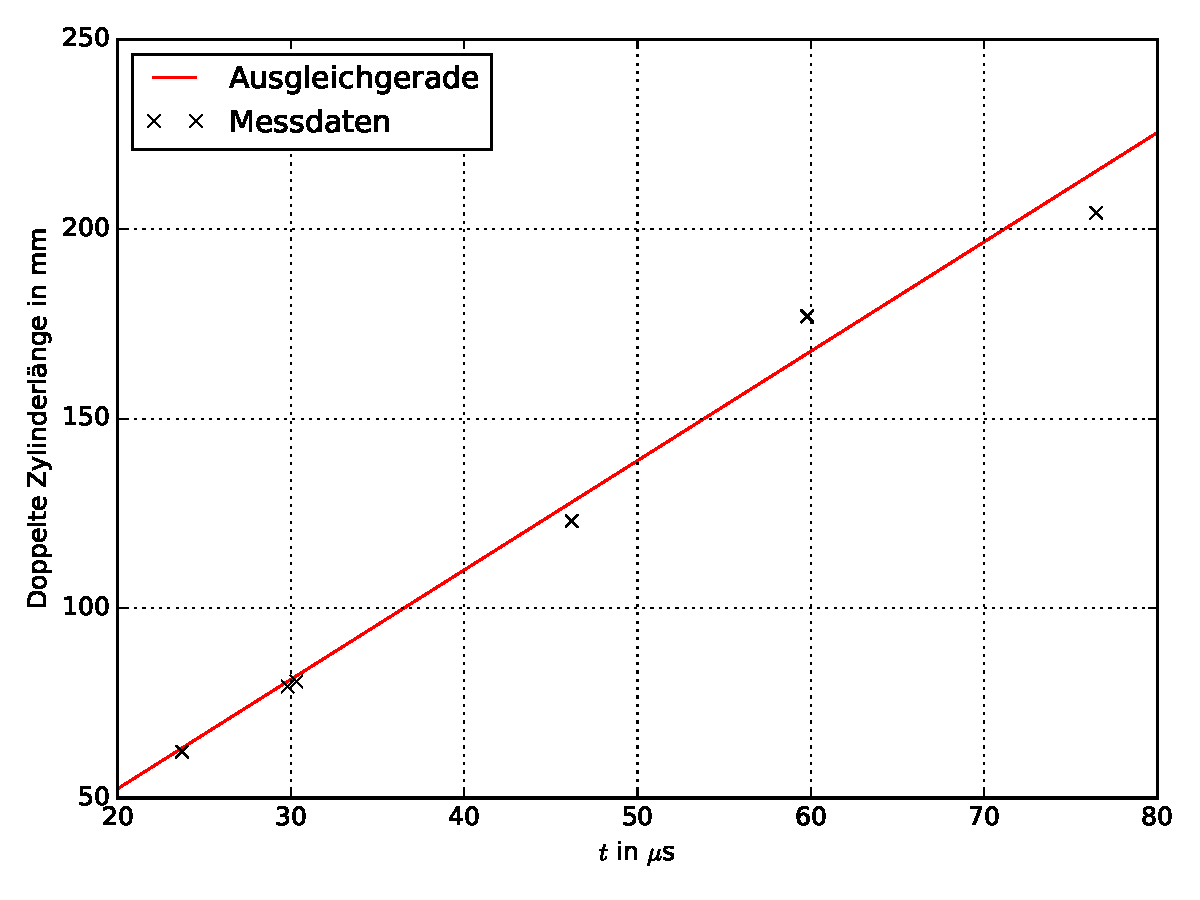
\includegraphics[width=\textwidth]{Pics/schallgesch_echo.pdf}
  \caption{Schallgeschwindigkeit in Acryl, bestimmt über das Impuls-Echo-Verfahren.}
  \label{fig:schallgesch_echo}
\end{figure}

\begin{table}
\centering
\caption{Messdaten zu dem Impuls-Echo-Verfahren. Die Werte sind den Zylindern 1 - 7 derReihe nach zuzuordnen. Der achte Messert entspricht einem Zylinder der Länge $\su{Z}_1 + \su{Z}_7$.}
\label{tab:Messdaten}
\begin{tabular}{S S S S}
\toprule
{$\su{U}\ua{1}$ in $\si{\volt}$} & {$t_1$ in $\si{\mu\second}$} & {$\su{U}\ua{2}$ in $\si{\volt}$} & {$t_2$ in $\si{\mu\second}$}  \\
\midrule
 0.90  & 0.40  & 0.17  & 30.30\\
0.97  & 0.40  & 0.02  & 59.80\\
0.98  & 0.50  & 0.01  & 59.80\\
1.00  & 0.40  & 0.12  & 76.49\\
0.97  & 0.40  & 0.25  & 23.70\\
0.98  & 0.50  & 0.19  & 29.80\\
0.97  & 0.40  & 0.04  & 46.20\\
1.00  & 0.50  & 0.12  & 75.70\\
\bottomrule
\end{tabular}
\end{table}

\FloatBarrier

\subsection{Bestimmung der Schallgeschwindigkeit mit dem Durchschallungsverfahren}

Die Messdaten zum Durchschallungsverfahren sind in Tabelle \ref{tab:durchschall}
dargestellt.
Es wurde gleich verfahren wie bei dem Impuls-Echo-Verfahren.

Die Werte ergeben sich zu:

\begin{align}
  \label{eqn:schallgesch_durch}
  c\ua{Acryl, durch} &= \SI{2878.377}{\meter\per\second} \\
  \Delta\ua{Sonde, durch} &= \SI{-2.946}{\meter\per\second}.
\end{align}

Das zugehörige Diagramm der Messung ist im Folgenden dargestellt.

\begin{figure}
  \centering
  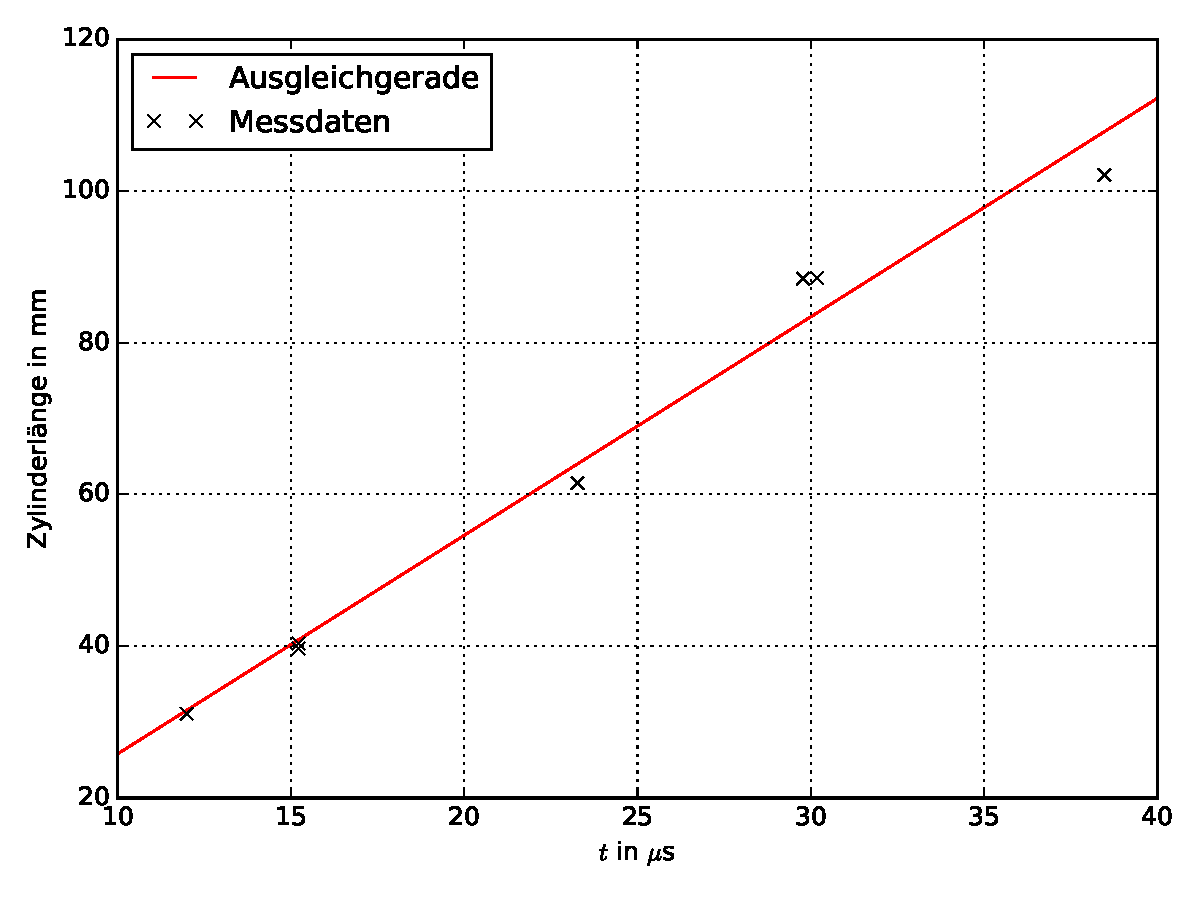
\includegraphics[width=\textwidth]{Pics/schallgesch_durch.pdf}
  \caption{Schallgeschwindigkeit in Acryl, bestimmt über das Durchschallungsverfahren.}
  \label{fig:schallgesch_durch}
\end{figure}

\begin{table}
\centering
\caption{Messdaten zu dem Durchschallungsverfahren. Die Messdaten sind der Reihe nach den Zylindern 1 - 7 zuzuordnen.}
\label{tab:durchschall}
\begin{tabular}{S }
\toprule
{Laufzeiten in \si{\mu\second}}  \\
\midrule
 15.21\\
29.78\\
30.18\\
38.48\\
11.98\\
15.21\\
23.27\\
\bottomrule
\end{tabular}
\end{table}

\FloatBarrier

\subsection{Spektrale Analyse und Cepstrum}

Die verwendeten Acrylplatten wurde mit einer Schieblehre vermessen.
Die Dicken wurden ebenfalls als fehlerfrei angenommen.

\begin{description}
  \item[Platte 1] $d_1 = \SI{9.9}{\milli\meter}$
  \item[Platte 2] $d_2 = \SI{6}{\milli\meter}$
\end{description}

Das Durchschallungsverfahren ergab die folgenden Werte.

\begin{description}
  \item[Platte 1] $d_1 = \SI{10.51}{\milli\meter}$
  \item[Platte 2] $d_2 = \SI{6.48}{\milli\meter}$
\end{description}

Die bestimmten Werte weichen um $\Delta\ua{Platte 1} = \SI{0.61}{\milli\meter}$
und $\Delta\ua{Platte 2} = \SI{0.48}{\milli\meter}$ von den mit der
Schieblehre vermessenen Werten ab.

Die Fehler aus dem systematische Fehler der Sonde sind vernachlässigbar klein.

Das Spektrum und das Cepstrum wurden aufgenommen. Die genommenen
Diagramme sind im Folgendem dargestellt.

\begin
{figure}
\centering
\begin{subfigure}{0.48\textwidth}
\centering
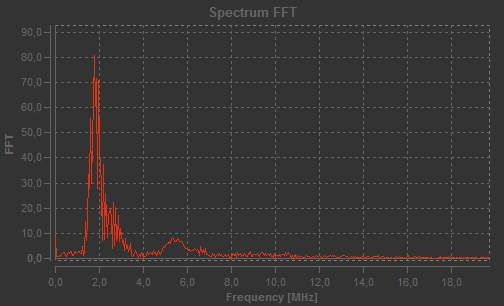
\includegraphics[height=4.2cm]{Pics/Z6_M3_S.jpg}
\caption{Aufgenommenes Spektrum.}
\label{fig:Spektrum}
\end{subfigure}
\begin
{subfigure}{0.48\textwidth}
\centering
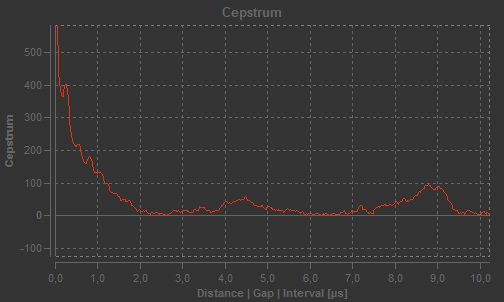
\includegraphics
[height=4.2cm]{Pics/Z6_M3_C.jpg}
\caption{Aufgenommenes Cepstrum.}
\label{fig:Cepstrum}
\end{subfigure}
\end{figure}

\subsection{Biometrische Untersuchung eines Augenmodells}

Es wurde ein Auge wie aus Abb. \ref{fig:Auge} untersucht.
Insgesamt wurden fünf Peaks aufgenommen die den folgenden Bestandteilen des Auges
zuzuordnen sind.

\begin{enumerate}
  \item Hornhaut
  \item Iris
  \item Linseneingang
  \item Linsenausgang
  \item Retina
\end{enumerate}

Die Peaks spiegeln der Aufzählung entsprechend die Bestandteilen des Auges wieder.
Für die Bereiche zwischen Hornhaut und Linseneingang, sowie
Linsenausgang und Retina wurde die Schallgeschwindigkeit für
Glaskörper verwendet ($c\ua{Glaskoerper} = \SI{1410}{\meter\per\second}$
\cite{anleitung01}).
Für den Bereich zwischen Linseneingang und Linsenausgang
wurde eine Schallgeschwindigkeit von $c\ua{Linse} = \SI{2500}{\meter\per\second}$
angenommen.

Die Bestandteile des Auges haben die folgenden Tiefen.

\begin{description}
  \item[Hornhaut] $\SI{0}{\milli\meter}$
  \item[Iris] $\SI{4.385(11)}{\milli\meter}$
  \item[Linseneingang] $\SI{7.635(18)}{\milli\meter}$
  \item[Linsenausgang] $\SI{14.835(21)}{\milli\meter}$
  \item[Retina] $\SI{44.23(9)}{\milli\meter}$
\end{description}

Die dazugehörigen Fehler entstehen durch den systematischen Fehler der Sonde.

Die Messdaten sind in der Tabelle \ref{tab:Auge} einzusehen.

\begin{table}
\centering
\caption{Messdaten zur biometrischen Untersuchung des Auges. Die Messdaten sind der Reihe den Bestandteile des Auges zuzuordnen.}
\label{tab:Auge} 
\begin{tabular}{S S }
\toprule
{Peakabstand $\Delta_{\symup{peak}}$ in \si{\mu\second}}  & {Absoluter Abstand}  \\
\midrule
 0.20  & 0.20\\
6.22  & 6.64\\
4.61  & 11.05\\
5.76  & 16.81\\
41.70  & 70.26\\
\bottomrule
\end{tabular}
\end{table}


\section{Diskussion}

Als Literaturwert der Schallgeschwindigkeit in Acryl wurde
$c\ua{Acyl, lit} = \SI{2730}{\meter\per\second}$\cite{lit} angenommen.
Die Schallgeschwindigkeit in Acryl wurde über zwei verschiedenen
Ultraschallverfahren ermittelt. Die berechneten Werte unterscheiden sich
um $\Delta\ua{c, gemessen} = \SI{1.740(917)}{\meter\per\second}$.
Hingegen liegt der Unterschied des gemittelten Wertes zum Literaturwert bei $\SI{149.246(3404)}{\meter\per\second}$.
Da beide Verfahren einen deutlichen Unterschied zu dem Literaturwert aufweisen,
aber untereinander kaum verschieden sind, wird
ein weiterer systematischer Fehler, der von dem systematischen Fehler der
Sonde verschieden ist angenommen.
Die Dicke der Acrylplatten wurden einmal über eine Schieblehre und
zum anderen über das Durchschallungsverfahren ermittelt.
Die Dicken, die sich aus dem Durchschallungsverfahren ergeben, sind
ca. einen halben Millimeter größer als die ausgemessenen Werte.
Mit dem Literaturwert für die Schallgeschwindigkeit von Acryl
ergeben sich die Plattendicken zu:

\begin{description}
  \item[Platte 1] $d_1 = \SI{9.96}{\milli\meter}$
  \item[Platte 2] $d_2 = \SI{6.14}{\milli\meter}$.
\end{description}

Damit ist die Abweichung der Plattendicken auf den systematischen Fehler
der Schallgeschwindigkeit zurückzuführen.

Die Diagramme aus der Spektralen Analyse (\ref{fig:Spektrum}, \ref{fig:Cepstrum})
werden im Folgenden diskutiert. In dem Diagramm des Cepstrums sind nicht die Lagen der tatsächlich
beobachteten Peaks erkenntlich, hingegen werden Peaks dargestellt, die
nicht beobachtet wurden. Das Spektrum zeigt einen Peak bei ca. $\SI{1.8}{\mega\hertz}$.
Die Eingangsfrequenz betrug hingegen $\SI{2}{\mega\hertz}$. Die weiteren Peaks
sind durch Reflexionen der Eingangswelle zu erklären.

Die biometrische Untersuchung des Auges ergab Werte, die
mit den Erwartungswerten übereinstimmen. Hierbei muss der
systematische Fehler ebenfalls bedacht werden, weshalb davon auszugehen
ist, dass die tatsächlichen Werte kleiner als die bestimmten Werte sind.


\printbibliography

\end{document}
